\chapter{immagini}
Un problema piuttosto complesso è la conversione di una immagine da analogica a digitale che, ovviamente, deve essere gestita tramite i pixel. Astraendo matematicamente un'immagine, infatti, è possibile trarre una matrice $M\times N$ che rappresenta i vari pixel ed i suoi coefficienti, ai fatti, rappresentano quali sfumature di colore verranno mostrate ed in quale posizione. Tuttavia se un'immagine di grigi è rappresentabile da un'unica matrice che avrà come coefficienti soltanto valori interi da un minimo di 0 ad un massimo di
255 ( 0 rappresenta il colore nero e 255 rappresenta il colore bianco), un'immagine a colore è ottenuta tramite la sovrapposizione di tre rappresentazioni della stessa immagine: una in scala di rossi, una in scala di verdi ed una in scala di blu; sarà quindi richiesto che il colore di ogni pixel di questa immagine sia rappresentato da vettore di tre valori, ciascuno per ogni intensità del colore rosso, verde e blu

\dfn{}{
    Sia $A\in \mathbb{R}^{M\times N}$ e sia $k\in \mathbb{N}$, diremo che: una matrice $B$ di dimensioni $(M+2k)\times (N+2k)$ \textbf{estende} la matrice $A$ se e solo se vale:
    \[
        \forall (i,j)\in \{\,\dots,M\}\times \{1,\dots, N\}. A_{(i,j)} = B_{(i+k, j+k)}
    \] 
}

Esempietto:
\esempio{
    
    \[A=  
        \begin{pmatrix}
            7&8&9\\
            12&13&14\\
            17&18&19
        \end{pmatrix}    
    \]
    Si può affermare che che la seguente matrice
    \[A=  
        \begin{pmatrix}
            1&2&3&4&5\\
            6&7&8&9&10\\
            11&12&13&14&15\\
            16&17&18&19&20\\
            21&22&23&24&25
        \end{pmatrix}    
    \]
    estende $A$, dove si ha $k=1$
}
Chiaramente, per ogni matrice ne esistono infinite che la estendono
\dfn{}{
    Sia $K\in\mathbb{R}^{D\times D}$ con $D$ dispari. Si definisce il \textbf{centro di matrice} della matrice $K$ come l'elemento di coordinate $(\frac{D+1}{2}, \frac{D+1}{2})$
}
\esempio{
    Sia la matrice di dimensioni $5\times 5$
    \[
       A=\begin{pmatrix}
        1&2&3&4&5\\
        6&7&8&9&10\\
        11&12&13&14&15\\
        16&17&18&19&20\\
        21&22&23&24&25
    \end{pmatrix} 
    \]
    
    Il suo centro di matrice è $(\frac{5+1}{2}, \frac{5+1}{2}): = 13$
}

\dfn{}{
    Sia $A\in\mathbb{R}^{M\times N}$ e sia $B\in\mathbb{R}^{(M+(D-1))\times (N+(D-1))}$ con $D$ dispari che estenda $A$. $\forall(i,j)\in\{1,\dots, M\}\times\{1,\dots, N\}$ si definisce $W_{(i,j)}\in\mathbb{R}^{D\times D}$ si definiscono \textbf{sotto-matrici} di $B$, il cui centro è $B_{(i + \frac{D-1}{2}, j + \frac{D-1}{2})}$
}
\esempio{
    Sia $A\in\mathbb{R}^{3\times 3}$
    
    \[
        \begin{pmatrix}
            7&8&9\\
            12&13 &14\\
            17&18&19
        \end{pmatrix}
    \]

    Occorre trovare una matrice $(3 + (D - 1)) \times (3 + (D - 1)) = (3 + 2) \times (3 + 2)$ che estenda $A$, ad esempio:
    \[
        \begin{pmatrix}
            1&2&3&4&5\\
            6&7&8&9&10\\
            11&12&13&14&15\\
            16&17&18&19&20\\
            21&22&23&24&25
        \end{pmatrix}
    \]

    ne segue che, per esempio, la matrice $W_{(1,3)}$ è la sotto-matrice di $B$, di dimensioni $3 \times 3$, il cui centro sia $B_{(2,4)}$. Di seguito:

    \[
        W_{(1,3)}  = \begin{pmatrix}
            3&4&5\\
            8&9&10\\
            13&14&15
        \end{pmatrix}    
    \]
}

\dfn{}{
    Sia $A\in \real^{M \times N}$ e $K\in\real^{D \times D}$, con $D$ un numero naturale dispari. Sia $B$ una matrice di dimensioni $(M + (D - 1)) \times (N + (D - 1))$ che estenda $A$. $\forall (i,j)\in \{1, … , M\} \times \{1, … , N\}$, siano $W_{(i,j)}$ le sotto-matrici di dimensione $D\times D$ definite precedentemente.

    Definiamo la matrice $C\in\real^{M\times N}$, come segue:
    \[
        \forall(i,j) \in    \{1, … , M\} \times \{1, … , N\}: C_{i,j} = \sum_{m=1}^{\frac{D-1}{2}}\sum_{n=1}^{\frac{D-1}{2}} K(m,n) W_{(i,j)}(m,n)
    \]
    Tale matrice $C$, che verrà anche denotata con $C = [K * A | B]$, è chiamata \textbf{convoluzione} di $K$ e $A$ rispetto all’estensione $B$

    All’interno del contesto di questa definizione, la matrice $K$ prenderà il nome di \textbf{nucleo} di convoluzione o kernel di convoluzione
}

\section{Estensione di una matrice}

\dfn{}{
    Sia $k$ un numero naturlae e $B$ una matrice di dimensioni $(M + 2k) \times (N + 2k)$. Definiamo la funzione:
    \[
        \mathcal{P}:\real^{M\times N}\to \real^{(M+2k)\times (N+2k)}\quad X\to \mathcal{P}(X)
    \]
    Tale che:
    \[
        \forall(i,j) \in    \{1, … , M\} \times \{1, … , N\}: X_{(i,j)} = \mathcal{P}(X)_{(i+k, j+k)}
    \]
    e:
    \begin{itemize}
        \item le prime $k$ colonne di $\mathcal{P}(X)$ siano uguali alle prime $k$ colonne di $B$
        \item le ultime $k$ colonne di $\mathcal{P}(X)$ siano uguali alle ultime $k$ colonne di $B$
        \item le prime $k$ righe di $\mathcal{P}(X)$ siano uguali alle prime $k$ righe di $B$
        \item le ultime $k$ righe di $\mathcal{P}(X)$ siano uguali alle ultime $k$ righe di $B$
    \end{itemize}
    La funzione $P$ così definita prenderà il nome di \textbf{patter di estensione di ordine $k$ rispetto alla matrice $B$}
}
È chiaro che, per come è definita la funzione $\mathcal{P}(X)$, questa estenderà sempre la matrice $X$

\dfn{}{
    Definiamo \textbf{funzione di convoluzione} la seguente:
    \[
        [K*(\cdot)|\mathcal{P}]:\real^{M\times N}\to \real^{M\times N} \quad X\to [K*X|\mathcal{P}(X)]   
    \]
    \begin{itemize}
        \item Dove $K$ è un nucleo di convoluzione di dimensioni $D\times D$ fissato
        \item $\mathcal{P}$ è un pattern di estensione di ordine $\frac{D-1}{2}$, rispetto ad una qualche matrice $B\in\real^{(M+(D+1)\times N + (D-1))}$, sempre fissata 
    \end{itemize}
}
\esempio{
    Si prendi come esempio tale immagine
    \begin{center}
        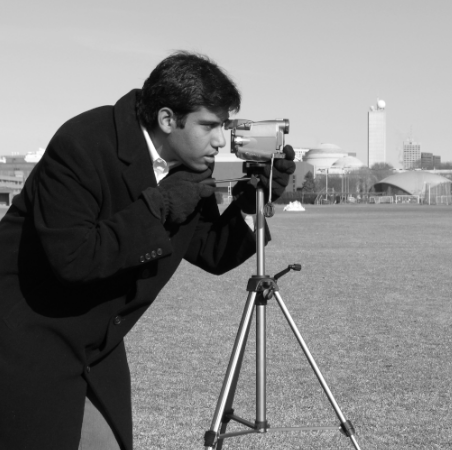
\includegraphics[width=7cm]{img/bro_foto.png}
    \end{center}
    E si supponi sia una matrice $A$ e si supponga tale matrice abbia, come nucleo di convoluzione $K$, tale matrice:
    \[
        K=\begin{pmatrix}
            0&\frac{1}{4}&0\\
            \frac{1}{4}&0&\frac{1}{4}\\
            0&\frac{1}{4}&0
        \end{pmatrix}    
    \]
    Ora non resta che svolgere la convoluzione in sè. 
    Ecco come:
    \begin{itemize}
        \item consideriamo una sotto-matrice $W$, sempre di dimensioni $D \times D$, della matrice $B$
        \item svolgiamo il prodotto scalare fra: la prima colonna di $W$ e la prima riga di $K$ , la seconda colonna di $W$ e la seconda riga di $K$ , così via fino alla \textit{D}-esima colonna di $W$ e alla \textit{D}-esima riga di $K$
        \item sommiamo tutti i prodotti scalari ottenuti
        \item il valore così determinato, diventerà il valore del pixel al centro della sotto-matrice $W$ considerata
        \item ripetere per tutte le sotto-matrici
        \item rimuovere le condizioni al bordo
    \end{itemize}
    \begin{center}
        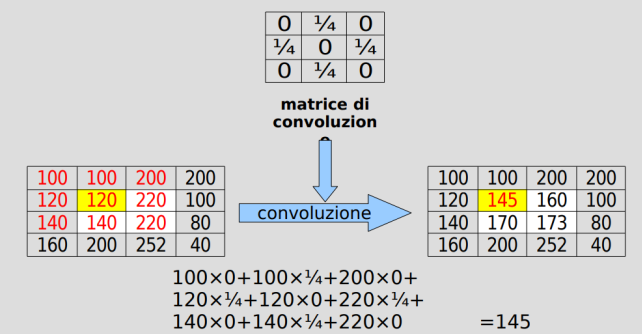
\includegraphics[width=7cm]{img/convoluzione_zio_pera.png}
    \end{center}
    In questo caso, il kernel utilizzato sostituisce il valore di ogni pixel con la media aritmetica dei valori contenuti nei quattro pixel ad esso adiacenti

    Ottenendo il seguente effetto di sfocatura:
    \begin{center}
        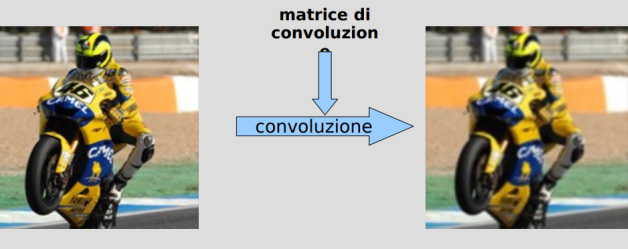
\includegraphics[width=7cm]{img/sfocatura.png}
    \end{center}

    Se si considera, invece, il seguente kernel:
    \[
      K = \begin{pmatrix}
            0&1&0\\
            1&-4&1 \\
            0&1&0
      \end{pmatrix}
    \]
    Osserviamo che, poiché la somma dei coefficienti è 0, sappiamo che se un pixel ha approssimativamente lo stesso colore dei quattro che gli sono adiacenti, allora verrà rimpiazzato da un valore prossimo a zero; in altre parole, il pixel diverrà di colore nero.
    Ne segue che tutti e soli i pixel che avranno un valore non nullo, saranno quelli posizionati in mezzo a due regioni di colori contrastanti. Pertanto, questo è un filtro che evidenzia i bordi dell’immagine
    \begin{center}
        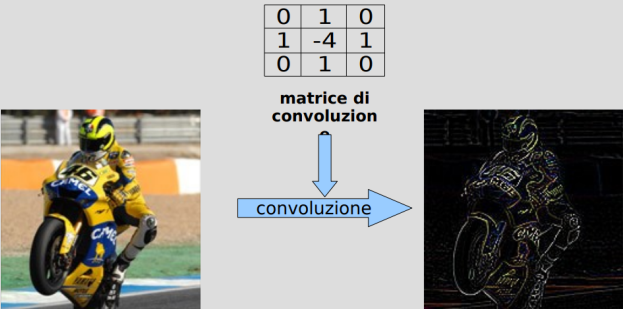
\includegraphics[width=7cm]{img/bordizzatura.png}
    \end{center}
}

\section{Point Spread Function}
Nel momento in cui un macchinario sensibile alla luce si accinge a fotografare, per esempio, ad una fonte luminosa puntiforme del tipo:
%TODO fai foto catso

Si ha che l'imagine ottenuta sarà:
%TODO fai foto dio pene

L'immagine che si ottiene è, quindi, un allargamento della fonte luminosa centrata nella fonte puntiforme. Questo fenomeno \red{è del tutto deterministico e legato all'apperacchiatura utilizzata per catturare l'immagine}. 

Sia $X$ la prima immagine e $Y$ la seconda, matematicamente si ha che:
\[
    A(X) = Y    
\]
Dove $\mathcal{A}$ è una funzione chiamata \textbf{Point Spread Function}. Ad essere più precisi riporterò qui la definizione di Point Spread Function
\dfn{}{
    Sia $x$ un immagine che rappresenta perfettamente il nostro
    oggetto originale. È definita $\mathcal{A}$ Point Spread Function, tale funzione:
    \[
        \mathcal{A}(x) = [K * x | \mathcal{P}]    
    \] 
    Dove $K$ è un kernel di convoluzione e $\mathcal{P}$ è un pattern di estensione
}

\subsection{PSF con errori non deterministici}
Tuttavia gli errori non deterministici non sono solo gli unici errori che corrompono le immagini, nel corso dell’acquisizione dell’immagine fenomeni aleatori e sostanzialmente imprevedibili danneggiano ulteriormente la nitidezza dell’immagine ottenuta.

Adesso sia $w$ un immagine i cui valori dei pixel siano stati selezionati aletoriamente secondo la distribuzione del rumore Gaussiano bianco. 

Si ha, quindi, un modello matematico \textbf{discreto} che spieghi come si sia formulata l'immagine $g$ (quella restituita dal nostro sistema di formazione di immagini), a partire da $x$, l'immagine che rappresenta veramente l'oggetto:
\[
    y^\delta = \mathcal{A}(x) + w =  [W*x|\mathcal{P}] + w  
\]
dove: 
\begin{itemize}
    \item $K$ è un qualche kernel di convoluzione
    \item $P$ è un pattern di estensione 
    \item $w$ è il medesimo di cui sopra
    \item $\mathcal{A}$ è la point spread function
\end{itemize}

Alternativamente si piò riscrivere il modello nella seguente forma matriciale:
\[
    y^\delta = Ax + w    
\]
Dove $A\in\real^{M\times N}$ che contiene le informazioni del nucleo
di convoluzione ed è tale che:
\[
    Ax = K * x
\]

Adesso ovviamente si vuole ardentemente sapere l'immagine originale $x$ zio pera
\subsubsection{Soluzione naive}
La soluzione naive è quella ottenuta risolvendo il problema di minimi quadrati:
\[
    min_x \|Ax-y^\delta\|_2^2    
\]
Essendo la matrice A di dimensione non molto piccola, calcolare la soluzione con la SVD è troppo costoso (ricordiamo che la complessità computazionale della fattorizzazione SVD è $O(4/3mn^2 )$ per una matrice di dimensione $m*n$). Quindi si risolvono le equazioni
normali:
\[
    A^TAx=A^Ty^\delta    
\]
Il sistema ha matrice simmetrica e definita positiva (supponiamo A di rango massimo) e per ragioni computazionali è conveniente utilizzare un metodo iterativo. Quindi  si applichiamo il CGLS al sistema delle equazioni normali
\subsection{Metriche di valutazione}
Le \textbf{metriche di valutazione} sono strumenti matematici utilizzati per quantificare la qualità di una ricostruzione, come nel caso della ricostruzione di un'immagine. Servono per confrontare un'immagine ottenuta (ricostruita) con il "ground truth" (l'immagine originale), con l'obiettivo di avere un numero che rappresenti quanto la ricostruzione sia accurata o fedele rispetto all'originale. Ci sono diverse metriche, proprio per avere diversi punti di vista
\subsubsection{errore relativo}
\dfn{}{
  siano $x_{GT}$ il "ground truth" e $x$ l'immagine ricostruita, viene definito l'errore relativo $ER$ tale valore:
  \[
        ER= \frac{\| x - x_{GT} \|_2^2}{\| x_{GT} \|_2^2}
  \]
}
\subsubsection{Rapporto Segnale-Rumore di Picco}
Prima di definire il Rapporto Segnale-Rumore di Picco occorre prima deifinire \textbf{l'errore quadratico medio} 
\dfn{}{
    Siano $M$ e $N$ le dimensioni dell'immagine, si definisce \textbf{ l'Errore Quadratico Medio} il seguente valore:
    \[
        MSE = \frac{\|x-x_{GT}\|_2^2}{MN}
    \]
}
Questo valore misura la differenza media al quadrato tra i pixel dell’immagine originale e quelli della ricostruzione. adesso si può introdurre il PSNR

\dfn{}{
    Sia $\max_{i,j}|x_{i,j}|$ è il valore massimo dell’immagine ricostruita (ad esempio, 255 per immagini in scala di grigi a 8 bit) e $MNE$ l'errore quadratico medio, si definisce \textbf{Rapporto Segnale-Rumore di Picco} tale valore:
    \[
        PSNR = 10 \cdot \log_{10}{(\frac{(\max_{i,j}|x_{i,j}|)^2}{MSE})}    
    \]
}
Un valore di PSNR più alto indica una qualità della ricostruzione migliore, perché significa che la differenza tra l'immagine ricostruita e l'originale è bassa

\subsubsection{Indice di Similarità Strutturale (SSIM)}
Il Structural Similarity Index (SSIM) è una metrica più complessa, progettata per essere più coerente con la percezione visiva umana. Considera non solo le differenze di intensità dei pixel, ma anche la struttura, luminanza e contrasto delle immagini. In altre parole, valuta quanto due immagini sono simili in termini di caratteristiche visive piuttosto che pixel per pixel. Più è vicino a uno, migliore è la qualità dell’immagine

\subsubsection{Roba}
\dfn{}{
    Sia \( A \) una matrice \( M \times N \), definiamo la funzione \( \mathcal{L} : \mathbb{R}^{M \times N} \rightarrow \mathbb{R}^{N \ast M} \) come segue:

\[
\mathcal{L}(A)
\]
è un vettore di dimensione \( N \ast M \), le cui:
\begin{itemize}
    \item prime \( N \) componenti sono la prima riga di \( A \), letta da sinistra a destra;
    \item seconde \( N \) componenti sono la seconda riga di \( A \), letta da sinistra a destra;
    \item \(\dots\)
    \item \( M \)-esime \( N \) componenti sono la \( M \)-esima riga di \( A \), letta da sinistra a destra.
\end{itemize}

Analogamente si definisce la conversione lessicografica per colonne.

}

\subsection{Regolarizzazione di Tikhonov applicata alle immagini}
Durante la soluzione di Naive si considerava il problema delle immagini come il seguente problema di minimo:
\[
    \min_x \|\|_2^2    
\]

Tuttavia dato che si ha un errore $y^\delta$ è necessario stabilizzare la funzione col metodo di regolarizzazione di Tikhonov:
\[
    \min_x \|Ax-y^\delta\|_2^2 + \lambda\|x^2\|_2^2
\]
Dove $\lambda$ è il parametro di Regolarizzazione. Applicando le condizioni del primo ordine $\nabla (f) = 0$ si ha:
\[
    (A^T A + \lambda I)x = A^T y^\delta    
\]

È possibile quindi risolvere il problema tramite il metodo CGLS
\subsubsection{Regolarizzazione con Variazione totale}
Una funzione di regolarizzazione alternativa a quella di Tikhonov e molto utilizzata nell’imaging è la funzione di Variazione Totale (TV) definita in questo modo:

\[
    TV(x) = \|\nabla (x)\|_1 = \sum_{i=1}^{M}\sum_{j=1}^{n} \sqrt{(x_{i+1,j}- x_{i,j})^2 + (x_{i,j+1 - x_{i,j}})^2}    
\]

La funzione $TV$ non è differenziabile nel punto $(0,0)$. Per ottenre la differenziabilità, si inserice un piccolo parametro $\beta > 0$:
\[
    TV^\beta(x) = \sum_{i=1}^{m}\sum_{j=1}^{n} \sqrt{(x_{i+1,j}- x_{i,j})^2 + (x_{i,j+1} - x_{i,j})^2 + \beta^2}
\]

Dove i valori di solito utilizzati per $\beta$ sono nell'ordine di $10^{-3}$

Il problema di regolarizzazione diventa quindi:
\[
    \min_x \|Ax-y^\delta\|_2^2 + \lambda TV ^ \beta(x)    
\]
Il metodo di regolarizzazione con TV ha il vantaggio di essere particolarmente efficace nell’eliminare il rumore e allo stesso tempo meglio preservare i contorni, anche in caso di basso rapporto segnale/rumore. Il suo uso è motivato dalla sua abilità nel recuperare le discontinuità nell’immagine, inoltre preserva i bordi dell’immagine rimuovendo piccoli dettagli come il rumore.
All’aumentare del parametro di regolarizzazione l’immagine tende a una immagine costante a tratti


